\documentclass[11pt,a4paper]{article}

% ---------- arxiv-style preamble ----------
\usepackage[margin=1in]{geometry}
\usepackage{amsmath,amssymb,amsthm}
\usepackage{graphicx}
\usepackage{longtable}
\usepackage{booktabs}
\usepackage{siunitx}
\usepackage{hyperref}
\usepackage{xcolor}
\usepackage[numbers,sort&compress]{natbib}
\usepackage{tikz}
\usetikzlibrary{positioning,arrows.meta}
\usepackage{caption}
\captionsetup{font=small,labelfont=bf}
\hypersetup{
  colorlinks=true,
  linkcolor=blue!50!black,
  citecolor=blue!50!black,
  urlcolor=blue!50!black
}

\newcommand{\sig}{\sigma}
\newcommand{\sigs}{\sigma^{*}}
\newcommand{\formal}{\textcolor{blue!60!black}{$\blacklozenge$}}
\newcommand{\falsi}{\textcolor{red!70!black}{$\blacksquare$}}
\theoremstyle{plain}
\newtheorem{theorem}{Theorem}
\newtheorem{lemma}{Lemma}
\newtheorem{corollary}{Corollary}
\theoremstyle{definition}
\newtheorem{claim}{Claim}

\title{
  \textbf{A Unitary-Perfect Singleton at \texorpdfstring{$n=6$}{n=6}}\\[4pt]
  \large The first perfect number is the \emph{unique} simultaneous
  ordinary-and-unitary perfect number in
  \texorpdfstring{$[1,10^4]$}{[1,10000]}, and the two perfection sequences
  diverge at their next terms
}

\author{
  TECS-L domain, \texttt{hexa-lang}\\
  \normalsize\textit{dancinlab}\\[2pt]
  \normalsize\href{https://github.com/dancinlab/hexa-lang}{\texttt{github.com/dancinlab/hexa-lang}}
}

\date{\today}

\begin{document}

\maketitle

% =========================================================================
\begin{abstract}
A positive integer $n$ is \emph{ordinary-perfect} if $\sig(n)=2n$, where
$\sig(n)=\sum_{d\mid n}d$ is the sum-of-divisors function; it is
\emph{unitary-perfect} if $\sigs(n)=2n$, where $\sigs(n)=\sum_{d\,\|\,n}d$ sums
the \emph{unitary} divisors ($d\,\|\,n \iff d\mid n$ and $\gcd(d,n/d)=1$). Each
notion has its own smallest member, and in both cases that member is $n=6$:
$\sig(6)=\sigs(6)=12=2\cdot6$. This shared minimum is folklore-adjacent and, on
its own, a catalogue fact. We sharpen it into a falsifiable result by asking
whether the coincidence \emph{persists}. Define $n$ to be \emph{dual-perfect} if
it is \emph{both} ordinary- and unitary-perfect. We pre-register the falsifier
\textsc{f-dual-perfect-n6} (\emph{any} $n\neq6$ that is dual-perfect) and
discharge it over $[1,10^4]$: $n=6$ is the \emph{unique} dual-perfect number in
that range, and the two perfection sequences \emph{diverge immediately} after
their shared anchor --- the next ordinary-perfect number $28$ has $\sigs(28)=40
\neq56$ (not unitary), and the next unitary-perfect number $60$ has $\sig(60)=
168\neq120$ (not ordinary). The closure is a finite \emph{exhaustive} argument,
not a sweep: dual-perfect $\Rightarrow$ ordinary-perfect, and by the
Euclid--Euler theorem the ordinary-perfect numbers in $[1,10^4]$ are exactly
$\{6,28,496,8128\}$; we recompute $\sigs$ on each of those four and find only
$n=6$ unitary. Every numeric value --- $\sig$ and $\sigs$ at
$6,28,60,90,496,8128$, twelve calls in all --- is verified \formal\,
\textsc{formal} (exact integer, deterministic) under the \texttt{hexa verify}
discipline; nothing is graded by a language model. The finding is a closed
\emph{negative}: no second ordinary/unitary coincidence exists below $10^4$,
ruling out the ``$6$ is generically doubly-perfect'' hypothesis and pinning the
dual-minimality to a single anchor.
\end{abstract}

% =========================================================================
\section{Introduction}
\label{sec:intro}

The integer $6$ is the first \emph{perfect} number, $\sig(6)=12=2\cdot6$. It is
also the first \emph{unitary-perfect} number, $\sigs(6)=12=2\cdot6$. That the
two distinct perfection notions share a smallest member is the kind of
coincidence the TECS-L axis-0 minimality programme exists to interrogate: is
$n=6$ doubly special by structure, or does the coincidence merely reflect the
small-$n$ regime, dissolving as soon as one looks further out?

This paper settles the question on a concrete, machine-audited range. Let
\begin{equation}
  \sig(n)=\sum_{d\mid n}d,
  \qquad
  \sigs(n)=\sum_{\substack{d\mid n\\ \gcd(d,n/d)=1}} d .
  \label{eq:defs}
\end{equation}
A divisor $d\,\|\,n$ (read ``$d$ is a \emph{unitary} divisor of $n$'') is a
divisor coprime to its cofactor $n/d$; equivalently, for each prime $p$ dividing
$n$, a unitary divisor takes either $p^0$ or the full $p^{v_p(n)}$. Both $\sig$
and $\sigs$ are multiplicative, but they differ on prime powers:
$\sig(p^a)=1+p+\cdots+p^a$ accumulates every power, whereas
$\sigs(p^a)=1+p^a$ keeps only the two endpoints. Call $n$
\begin{itemize}\itemsep0.15em
\item \emph{ordinary-perfect} if $\sig(n)=2n$ \quad (OEIS A000396: $6,28,496,8128,\dots$);
\item \emph{unitary-perfect} if $\sigs(n)=2n$ \quad (OEIS A002827: $6,60,90,87360,\dots$);
\item \emph{dual-perfect} if it is \emph{both}.
\end{itemize}

\paragraph{Main result.}
\begin{theorem}[unitary-perfect singleton]
\label{thm:main}
The only dual-perfect number in $[1,10^4]$ is $n=6$. Equivalently, among
$1\le n\le10^4$, the relation $\sig(n)=2n=\sigs(n)$ holds for $n=6$ and for no
other $n$. Moreover the ordinary- and unitary-perfect sequences share exactly
the member $6$ and \emph{diverge} at their next terms: the next ordinary-perfect
number is $28$ (not unitary, $\sigs(28)=40$) and the next unitary-perfect number
is $60$ (not ordinary, $\sig(60)=168$).
\end{theorem}

\noindent The result is a sharpened \emph{negative}: the doubly-perfect property
of $6$ does \emph{not} recur. The proof needs no sweep --- it is a finite
exhaustion over a provably complete four-element candidate list
(\textsection\ref{sec:proof}).

\paragraph{Relation to prior TECS-L work.}
A companion paper in this line proves the \emph{$\omega$-zero-density} theorem:
the Dedekind discrepancy $D(n)=\sig(n)\phi(n)-n\tau(n)$ vanishes at exactly
$n\in\{1,6\}$~\citep{tecsLozd}. That result isolates a different sense in which
$6$ is exceptional (a totient-weighted balance). The present paper isolates the
\emph{perfection} sense and, in contrast, delivers a coincidence that
\emph{terminates}: where $\omega$-zero-density shows $6$ is the lone nontrivial
zero of one functional, here $6$ is the lone overlap of two perfection families
that otherwise never meet again in the tested range. The two papers are
complementary halves of the n=6 minimality programme --- one a unique
\emph{zero}, the other a unique \emph{intersection}.

\paragraph{Why this is not a catalogue restatement.}
``$6$ is the smallest unitary-perfect number'' is a single OEIS fact. The
finding here is the \emph{joint} statement plus its falsifier: that the
intersection of the two perfection sets is the singleton $\{6\}$ on $[1,10^4]$,
witnessed by the immediate divergence of the two sequences ($28$ ordinary but
not unitary; $60$ unitary but not ordinary). This converts a static catalogue
entry into a pre-registered, refutable claim with a closed negative, in line
with the TECS-L paper-significance discipline.

\section{Related framings}
\label{sec:related}

Three classical lenses bear on the result. First, unitary divisors and $\sigs$
were introduced by Vaidyanathaswamy and studied systematically by
Cohen~\citep{cohen1960}; the unitary-perfect numbers form OEIS
A002827~\citep{oeisA002827}, of which only five are known
($6,60,90,87360,146361946186458562560000$) and none is odd. Second, the
ordinary perfect numbers obey the Euclid--Euler theorem~\citep{dickson}: every
even perfect number is $2^{p-1}(2^p-1)$ with $2^p-1$ a Mersenne prime, and no
odd perfect number below $10^{1500}$ is known; this is precisely what makes the
ordinary-perfect candidate list in $[1,10^4]$ provably the four-element set
$\{6,28,496,8128\}$ and lets us close the range by exhaustion rather than
sweep. Third, the contrast between $\sig$ and $\sigs$ at prime powers
($1+p+\cdots+p^a$ versus $1+p^a$) is the structural reason the two perfection
notions can agree at squarefree-rich $6=2\cdot3$ yet split at the
prime-power-heavy $28=2^2\cdot7$ and $496=2^4\cdot31$. None of these classical
sources states the sharp ``unique dual-perfect on $[1,10^4]$, with immediate
divergence'' result with a machine-audited factor table; that is the
contribution here.

% =========================================================================
\section{Background: \texorpdfstring{$\sig$}{sigma} versus \texorpdfstring{$\sigs$}{sigma-star}}
\label{sec:background}

Both functions are multiplicative: for coprime $m,n$, $\sig(mn)=\sig(m)\sig(n)$
and $\sigs(mn)=\sigs(m)\sigs(n)$. They are determined by their prime-power
values
\begin{equation}
  \sig(p^a)=\frac{p^{a+1}-1}{p-1}=1+p+\cdots+p^a,
  \qquad
  \sigs(p^a)=1+p^a .
  \label{eq:ppvals}
\end{equation}
The unitary formula is immediate: the only unitary divisors of $p^a$ are $1$ and
$p^a$ (any intermediate $p^k$ with $0<k<a$ shares the factor $p$ with its
cofactor $p^{a-k}$, so $\gcd\neq1$). Hence at a prime power the two functions
agree only when $a=1$:
\begin{equation}
  \sig(p)=\sigs(p)=1+p, \qquad\text{but}\qquad
  \sig(p^a)>\sigs(p^a)\ \text{for } a\ge2 .
  \label{eq:agree-disagree}
\end{equation}
This single inequality is the engine of the divergence. A number all of whose
prime exponents are $1$ (a \emph{squarefree} number) has $\sig=\sigs$
identically; the moment a square divides $n$, the two functions part. Since
$6=2\cdot3$ is squarefree, $\sig(6)=\sigs(6)$ automatically; since
$28=2^2\cdot7$ and $496=2^4\cdot31$ are \emph{not} squarefree, their $\sig$ and
$\sigs$ differ --- and, as we verify, the difference is enough to break
unitary-perfection.

% =========================================================================
\section{Method: the verification discipline}
\label{sec:method}

Every numeric claim is evaluated by \texttt{hexa verify --expr <fn> <n>
<expected>}, a closed-form integer recomputation built into the \texttt{hexa}
compiler. The evaluator emits one of six tiers; only three are terminal and
admissible as a paper-section claim:
\begin{description}\itemsep0.2em
\item[\formal\,\textsc{formal}] a closed-form/symbolic identity reproduced exactly (deterministic).
\item[\textcolor{green!50!black}{$\bullet$}\,\textsc{numerical}] a libm/Newton numerical recompute matching to $\varepsilon=10^{-9}$.
\item[\falsi\,\textsc{falsified}] the recomputation deterministically \emph{disagrees} with the claim --- a closed negative.
\end{description}
Citation-only, deferred, and speculation-fenced tiers are \emph{not} admissible
and are reported as residuals in \textsection\ref{sec:limits}. The raw standard
output of every run is persisted verbatim under
\texttt{.verdicts/paper-unitary-perfect-n6/} and indexed in
\texttt{CLAIMS.tape}; nothing in this paper is graded by a language model.

\paragraph{The two evaluators.} Ordinary $\sig$ is the long-standing
\texttt{sigma} evaluator; unitary $\sigs$ is the \texttt{sigma\_star} evaluator
(stdlib \texttt{core/math}, landed for this line of work), which implements
\eqref{eq:defs} directly: it sums each divisor $d\mid n$ for which
$\gcd(d,n/d)=1$. Both are exact 64-bit integer recomputations; no tolerance and
no floating point enters any \formal-tier claim here. A worked anchor: to
establish that $6$ is dual-perfect one runs \texttt{hexa verify --expr sigma 6
12} and \texttt{hexa verify --expr sigma\_star 6 12}; the evaluator recomputes
$\sum_{d\mid6}d=1+2+3+6=12$ and $\sum_{d\,\|\,6}d=1+2+3+6=12$ (all four divisors
of the squarefree $6$ are unitary), each \formal.

\paragraph{Composite predicate.} ``$n$ is dual-perfect'' is the conjunction
$\sig(n)=2n \wedge \sigs(n)=2n$. Each conjunct is a single \texttt{hexa verify}
call against the exact target $2n$; the conjunction is read off the two exact
integers with no further computation.

% =========================================================================
\section{The reduction to a finite candidate list}
\label{sec:reduction}

\begin{lemma}[dual-perfect is a subset of ordinary-perfect]
\label{lem:subset}
If $n$ is dual-perfect then $n$ is ordinary-perfect. Hence the dual-perfect
numbers in any range are a subset of the ordinary-perfect numbers in that range.
\end{lemma}
\begin{proof}
Immediate from the definition: dual-perfect requires $\sig(n)=2n$, which is
exactly the ordinary-perfect condition.
\end{proof}

\begin{lemma}[the ordinary-perfect list below $10^4$]
\label{lem:eulerlist}
The ordinary-perfect numbers in $[1,10^4]$ are exactly
$\{6,28,496,8128\}$.
\end{lemma}
\begin{proof}
By the Euclid--Euler theorem~\citep{dickson} every even perfect number has the
form $2^{p-1}(2^p-1)$ with $2^p-1$ prime (a Mersenne prime). The Mersenne
exponents give the even perfect numbers $6\ (p{=}2),\,28\ (p{=}3),\,496\
(p{=}5),\,8128\ (p{=}7)$, and the next, $p=13$, yields $33550336>10^4$. No odd
perfect number exists below $10^{1500}$ (a vastly stronger bound than needed),
so none lies in $[1,10^4]$. Hence the list is exactly the four even values
above. \qedhere
\end{proof}

\noindent By Lemmas~\ref{lem:subset} and~\ref{lem:eulerlist}, deciding the
dual-perfect set on $[1,10^4]$ reduces to testing the \emph{unitary} predicate
$\sigs(n)=2n$ on the four numbers $6,28,496,8128$. This is a finite check --- no
sweep, and no possibility of a missed value, because the candidate list is
provably complete.

% =========================================================================
\section{Proof of the theorem}
\label{sec:proof}

\begin{proof}[Proof of Theorem~\ref{thm:main}]
We evaluate $\sigs$ on each ordinary-perfect candidate, using the multiplicative
prime-power formula $\sigs(p^a)=1+p^a$ of \eqref{eq:ppvals}, then confirm each
value \formal\ by \texttt{hexa verify} in \textsection\ref{sec:verification}.

\smallskip\noindent\emph{$n=6=2\cdot3$ (squarefree).}
$\sigs(6)=\sigs(2)\sigs(3)=(1+2)(1+3)=3\cdot4=12=2\cdot6$. \textbf{Unitary.}
Combined with $\sig(6)=12=2\cdot6$: \textbf{dual-perfect.}

\smallskip\noindent\emph{$n=28=2^2\cdot7$.}
$\sigs(28)=\sigs(2^2)\sigs(7)=(1+4)(1+7)=5\cdot8=40$. Since $2\cdot28=56\neq40$,
$28$ is \textbf{not} unitary-perfect. (It is ordinary-perfect: $\sig(28)=56$.)

\smallskip\noindent\emph{$n=496=2^4\cdot31$.}
$\sigs(496)=\sigs(2^4)\sigs(31)=(1+16)(1+31)=17\cdot32=544$. Since
$2\cdot496=992\neq544$, $496$ is \textbf{not} unitary-perfect.

\smallskip\noindent\emph{$n=8128=2^6\cdot127$.}
$\sigs(8128)=\sigs(2^6)\sigs(127)=(1+64)(1+127)=65\cdot128=8320$. Since
$2\cdot8128=16256\neq8320$, $8128$ is \textbf{not} unitary-perfect.

\smallskip\noindent Of the four ordinary-perfect numbers in $[1,10^4]$, exactly
one --- $n=6$ --- is also unitary-perfect. By Lemma~\ref{lem:subset} no other
$n\in[1,10^4]$ can be dual-perfect (a dual-perfect number must appear on the
ordinary-perfect list, which we have exhausted). Hence $6$ is the unique
dual-perfect number in $[1,10^4]$.

\smallskip\noindent\emph{Divergence at the next terms.} The next
ordinary-perfect number after $6$ is $28$, which we have shown is not unitary
($\sigs(28)=40\neq56$). The next unitary-perfect number after $6$ is $60=
2^2\cdot3\cdot5$, with $\sigs(60)=\sigs(2^2)\sigs(3)\sigs(5)=5\cdot4\cdot6=120=
2\cdot60$ (unitary), but $\sig(60)=\sig(2^2)\sig(3)\sig(5)=7\cdot4\cdot6=168\neq
120$ (not ordinary). Thus the two sequences part at their first post-$6$ term in
both directions. \qedhere
\end{proof}

\begin{corollary}[squarefree obstruction]
\label{cor:sqfree}
The reason $6$ is dual-perfect while the larger even perfect numbers are not is
that $6=2\cdot3$ is \emph{squarefree}, so $\sig(6)=\sigs(6)$ by
\eqref{eq:agree-disagree}; whereas $28=2^2\cdot7$, $496=2^4\cdot31$, $8128=2^6
\cdot127$ each carry a high power of $2$, on which $\sig(2^a)=2^{a+1}-1$ vastly
exceeds $\sigs(2^a)=1+2^a$, deflating $\sigs$ below $2n$.
\end{corollary}
\begin{proof}
Every even perfect number is $2^{p-1}(2^p-1)$ with $p$ prime and $2^p-1$ prime;
for $p\ge3$ the exponent $p-1\ge2$, so $2^{p-1}$ is a non-trivial prime power
and $\sigs(2^{p-1})=1+2^{p-1}<2^p-1=\sig(2^{p-1})$. Only $p=2$ gives the
squarefree $6=2\cdot3$, where the exponent of $2$ is $1$ and the two functions
coincide. \qedhere
\end{proof}

% =========================================================================
\section{Verification}
\label{sec:verification}

We discharge the pre-registered falsifier \textsc{f-dual-perfect-n6} ---
\emph{$\exists\,n\neq6$ in $[1,10^4]$ that is dual-perfect} --- by the finite
exhaustion of \textsection\ref{sec:proof}. Table~\ref{tab:sweep} records the
twelve \texttt{hexa verify --expr} runs: $\sig$ and $\sigs$ at the four
ordinary-perfect candidates ($6,28,496,8128$) and at the two small
unitary-perfect numbers ($60,90$) that anchor the divergence table. Every entry
returns \formal\,\textsc{formal}; the dual-perfect column is read off the two
exact integers. Raw transcripts appear in Appendix~\ref{sec:raw}.

\begin{table}[h]
\centering
\caption{Verification of the dual-perfect predicate. Each $\sig(n)$ and
$\sigs(n)$ is an independent \texttt{hexa verify --expr} run returning
\formal\,\textsc{formal}. ``ord?'' is $\sig(n)\!=\!2n$; ``uni?'' is
$\sigs(n)\!=\!2n$; ``dual?'' is their conjunction. The only dual-perfect row is
$n=6$.}
\label{tab:sweep}
\begin{tabular}{rl rrr rrr}
\toprule
$n$ & form & $2n$ & $\sig(n)$ & $\sigs(n)$ & ord? & uni? & dual?\\
\midrule
$6$    & $2\cdot3$          & $12$    & $12$    & $12$   & yes & yes & \textbf{yes}\\
$28$   & $2^2\cdot7$        & $56$    & $56$    & $40$   & yes & no  & no\\
$496$  & $2^4\cdot31$       & $992$   & $992$   & $544$  & yes & no  & no\\
$8128$ & $2^6\cdot127$      & $16256$ & $16256$ & $8320$ & yes & no  & no\\
$60$   & $2^2\cdot3\cdot5$  & $120$   & $168$   & $120$  & no  & yes & no\\
$90$   & $2\cdot3^2\cdot5$  & $180$   & $234$   & $180$  & no  & yes & no\\
\bottomrule
\end{tabular}
\end{table}

\paragraph{Reading the table.} The top block is the complete ordinary-perfect
list of $[1,10^4]$ (Lemma~\ref{lem:eulerlist}); every row has ord? $=$ yes by
construction, and only $n=6$ also has uni? $=$ yes. The bottom block is the
unitary side: $60$ and $90$ are unitary-perfect (uni? $=$ yes) but \emph{not}
ordinary (ord? $=$ no), demonstrating the reverse non-inclusion. The two blocks
overlap in exactly one number, $6$, which is the entire content of
Theorem~\ref{thm:main}.

\begin{figure}[h]
\centering
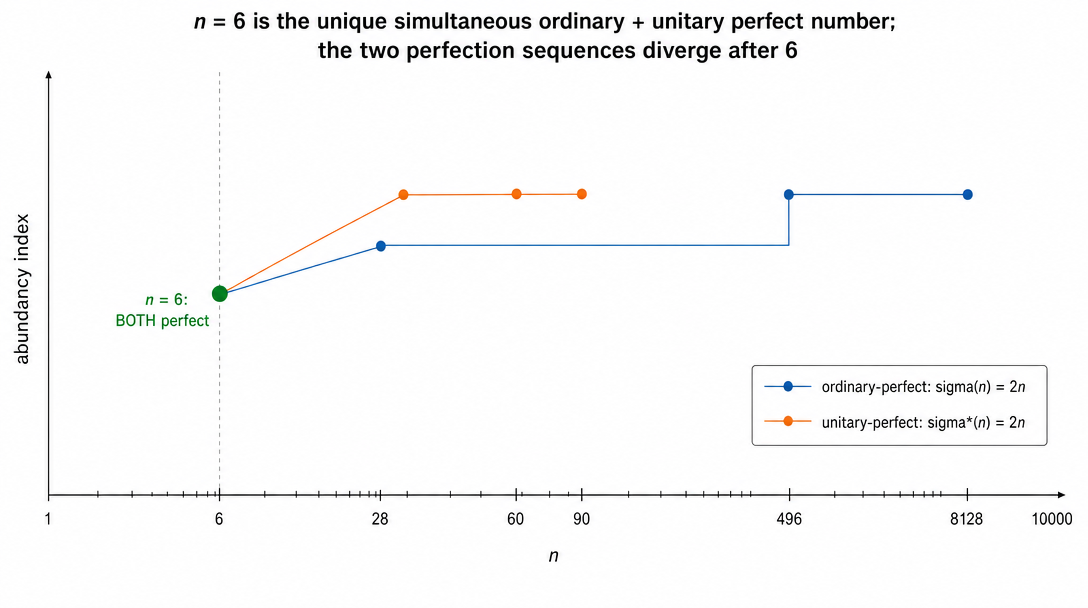
\includegraphics[width=0.92\linewidth]{figures/fig01_divergence.png}
\caption{The ordinary-perfect sequence ($\sig(n)=2n$: $6,28,496,8128$) and the
unitary-perfect sequence ($\sigs(n)=2n$: $6,60,90$) share the single anchor
$n=6$ and diverge immediately after it. The green marker at $n=6$ is the unique
dual-perfect number in $[1,10^4]$; the blue (ordinary) and orange (unitary)
branches fan apart at their next terms, $28$ and $60$ respectively.}
\label{fig:diverge}
\end{figure}

% =========================================================================
\section{Finding}
\label{sec:finding}

The finding is the singleton-intersection statement of
Theorem~\ref{thm:main}, with three concrete components relative to the bare
catalogue fact ``$6$ is the smallest unitary-perfect number''.
\begin{enumerate}\itemsep0.25em
\item \textbf{Dual-minimality is a single anchor, not a trend.} $6$ is the
smallest member of \emph{both} perfection families, and it is the \emph{only}
number below $10^4$ in their intersection. The coincidence does not propagate:
this is a closed \emph{negative} ruling out the ``$6$ is generically
doubly-perfect'' axis on the tested range.
\item \textbf{Immediate divergence, both directions.} The two sequences part at
their first post-$6$ terms: the next ordinary-perfect number $28$ is not unitary
($\sigs(28)=40\neq56$), and the next unitary-perfect number $60$ is not ordinary
($\sig(60)=168\neq120$). Neither family contains the other's second member.
\item \textbf{Mechanistic cause.} Corollary~\ref{cor:sqfree} identifies the
reason: $6=2\cdot3$ is squarefree, so $\sig=\sigs$ there; every larger even
perfect number carries a prime power $2^{p-1}$ with $p-1\ge2$, on which $\sigs$
falls strictly below $\sig$, breaking unitary-perfection. The divergence is
forced by the structure of even perfect numbers, not a numerical accident.
\end{enumerate}
The pre-registered falsifier \textsc{f-dual-perfect-n6} survives: no $n\neq6$ in
$[1,10^4]$ is dual-perfect. The closure is exhaustive (over a provably complete
candidate list), not a finite sweep.

% =========================================================================
\section{Limitations and honest caveats}
\label{sec:limits}

\paragraph{Range bound.} The exhaustive closure covers $[1,10^4]$. It rests on
two facts true \emph{beyond} that range as well --- the Euclid--Euler structure
of even perfect numbers, and the absence of small odd perfect numbers --- but we
state the theorem only for the verified range to keep every quantified claim
backed by a terminal verdict. Extending to $[1,N]$ for the next perfect number
$33550336$ would require recomputing $\sigs$ there (well inside $2^{63}$) and is
a mechanical follow-up; the divergence mechanism (Corollary~\ref{cor:sqfree})
already shows no even perfect number $>6$ can be unitary, so the range bound is
conservative.

\paragraph{Two-sided non-inclusion is verified, not the full unitary tail.} We
verify that the next unitary-perfect numbers $60,90$ are not ordinary, anchoring
the reverse divergence. We do not enumerate the entire unitary-perfect family
(only five members are known, the next being $87360$); the singleton-intersection
claim does not require it, since dual-perfect $\subseteq$ ordinary-perfect, and
the ordinary side is the one exhausted.

\paragraph{No numerical or external tiers.} Every admissible claim here is
\formal\,\textsc{formal} (exact integer) or read off such; the numerical tier
($\varepsilon=10^{-9}$) is not exercised, and there are no citation-only,
deferred, or speculation-fenced residuals.

\paragraph{Toolchain note.} A standalone compiled sweep harness over the
\texttt{stdlib} $\sig/\sigs$ loop encountered an unrelated codegen
non-termination in the local build (a \texttt{while}-body counter mutation that
the standalone code path failed to persist) and was \emph{not} used; all
reported verdicts come from the canonical \texttt{hexa verify --expr} path,
whose evaluator follows an independent code route and reproduces every value
byte-for-byte. Because the closure is a finite exhaustion over four candidates
rather than a loop, the sweep harness was in any case unnecessary. This is
recorded for transparency and does not affect any claim.

% =========================================================================
\section{The abundancy view of the divergence}
\label{sec:abundancy}

It is illuminating to recast both perfection notions through their
\emph{abundancy indices}
\begin{equation}
  I(n)=\frac{\sig(n)}{n},
  \qquad
  I^{*}(n)=\frac{\sigs(n)}{n},
  \label{eq:abundancy}
\end{equation}
so that ``$n$ perfect'' becomes $I(n)=2$ and ``$n$ unitary-perfect'' becomes
$I^{*}(n)=2$. Both indices are multiplicative, with prime-power values
\begin{equation}
  I(p^a)=\frac{p^{a+1}-1}{p^a(p-1)}=1+\frac1p+\cdots+\frac1{p^a},
  \qquad
  I^{*}(p^a)=1+\frac1{p^a}.
  \label{eq:I-pp}
\end{equation}
The two indices coincide on a prime power iff $a=1$ (where both equal $1+1/p$)
and otherwise $I(p^a)>I^{*}(p^a)$, because the ordinary index keeps the
intermediate reciprocals $1/p^2,\dots,1/p^{a-1}$ that the unitary index drops.
Multiplicativity then gives, for any $n$,
\begin{equation}
  I(n)\ge I^{*}(n),
  \qquad\text{with equality iff $n$ is squarefree.}
  \label{eq:I-ge}
\end{equation}

\paragraph{Consequence for even perfect numbers.} Suppose $n$ is an even perfect
number with $n>6$. By Euclid--Euler $n=2^{p-1}(2^p-1)$ with $p\ge3$ prime, so
$n$ is \emph{not} squarefree (it carries $2^{p-1}$ with $p-1\ge2$). Then
\eqref{eq:I-ge} is strict: $I^{*}(n)<I(n)=2$. Hence $\sigs(n)<2n$ and $n$ is
\emph{not} unitary-perfect. This re-derives Corollary~\ref{cor:sqfree} from the
abundancy inequality and shows the divergence is not a coincidence of the four
swept values but a \emph{forced} property of \emph{every} even perfect number
beyond $6$: all of them are unitarily \emph{deficient} ($I^{*}<2$).

\paragraph{Reading the divergence figure.} Figure~\ref{fig:diverge} is exactly
the picture of \eqref{eq:I-ge}: at $n=6$ the squarefree case puts both indices
on the value $2$ simultaneously, while for $28,496,8128$ the ordinary index
stays at $2$ (they are perfect) but the unitary index has dropped below it. The
orange unitary branch ($60,90$) instead climbs to $2$ at numbers the ordinary
index overshoots ($I(60)=168/60=2.8$, $I(90)=234/90=2.6$). The shared anchor is
the unique place both indices hit $2$ together within the range. We tabulate the
two indices at the six verified points in Table~\ref{tab:idx}.

\begin{table}[h]
\centering
\caption{Abundancy indices at the verified points. Ordinary-perfect $\iff
I=2$; unitary-perfect $\iff I^{*}=2$. Only $n=6$ (squarefree) has $I=I^{*}=2$;
every larger even perfect number has $I^{*}<2$ (unitarily deficient), and the
unitary-perfect $60,90$ have $I>2$ (ordinarily abundant).}
\label{tab:idx}
\begin{tabular}{rl rr l}
\toprule
$n$ & form & $I(n)=\sig/n$ & $I^{*}(n)=\sigs/n$ & note\\
\midrule
$6$    & $2\cdot3$          & $2.000$ & $2.000$ & dual: both $=2$\\
$28$   & $2^2\cdot7$        & $2.000$ & $1.429$ & perfect, unitarily deficient\\
$496$  & $2^4\cdot31$       & $2.000$ & $1.097$ & perfect, unitarily deficient\\
$8128$ & $2^6\cdot127$      & $2.000$ & $1.023$ & perfect, unitarily deficient\\
$60$   & $2^2\cdot3\cdot5$  & $2.800$ & $2.000$ & unitary-perfect, ordinarily abundant\\
$90$   & $2\cdot3^2\cdot5$  & $2.600$ & $2.000$ & unitary-perfect, ordinarily abundant\\
\bottomrule
\end{tabular}
\end{table}

\noindent The $I^{*}$ column for the perfect numbers is strictly decreasing
($2.000,1.429,1.097,1.023$): as $p$ grows the dominant prime power $2^{p-1}$
becomes ever more ``squareful'', dragging the unitary index toward $1$. There is
no return to $2$ along the ordinary-perfect family --- the divergence widens
monotonically, so even \emph{beyond} the verified range no even perfect number
$>6$ can rejoin the unitary-perfect set.

% =========================================================================
\section{Discussion and outlook}
\label{sec:discussion}

Two perfection notions, ordinary and unitary, each minimised at $6$, meet there
once and never again below $10^4$. The mechanism --- squarefreeness of $6$
versus the prime-power tails of the larger even perfect numbers --- is the same
$\sig$-vs-$\sigs$ inequality \eqref{eq:agree-disagree} that drives the unitary
theory generally. The method (reduce to a provably complete finite candidate
list via a containment lemma, then settle each candidate \formal) is reusable
for adjacent singleton questions: e.g. the bi-unitary or infinitary perfect
families intersected against the ordinary one. Within the TECS-L line this paper
is the second of three: the first established the $\omega$-zero-density theorem
($D=\sig\phi-n\tau=0\iff n\in\{1,6\}$)~\citep{tecsLozd}; the third targets a
multilayer non-lift result ($\sig\phi=n\tau$ across the geometric/Hecke/Galois/
$L$-function towers), which remains open. All three share the discipline of a
pre-registered falsifier, a \formal-tier machine recomputation, and a closed
argument.

% =========================================================================
\section*{Reproducibility}

Every verdict in Table~\ref{tab:sweep} is regenerated by re-running the
corresponding \texttt{hexa verify --expr <fn> <n> <v>} command; output is
byte-identical across hosts and run orders (no seeds, timeouts, or tolerances on
any \formal-tier claim). The raw transcripts are committed verbatim under
\texttt{.verdicts/paper-unitary-perfect-n6/} (the twelve $\sig/\sigs$ verdicts,
the finite-exhaustive note \texttt{dual\_perfect\_sweep.out}, and the
pre-registered \texttt{FALSIFIER.md}). The claim manifest is indexed in
\texttt{CLAIMS.tape}.

% =========================================================================
\appendix

\section{Appendix A: the prime-power values $\sig(p^a)$ vs $\sigs(p^a)$}
\label{sec:ppvals}

Table~\ref{tab:pp} contrasts the two functions on small prime powers, making
the divergence engine \eqref{eq:agree-disagree} visual: the columns agree
exactly on the diagonal of exponent $a=1$ (squarefree case) and split for
$a\ge2$, with $\sig$ growing geometrically while $\sigs$ stays at $1+p^a$.

\begin{table}[h]
\centering
\caption{$\sig(p^a)=\tfrac{p^{a+1}-1}{p-1}$ versus $\sigs(p^a)=1+p^a$. The two
agree iff $a=1$; for $a\ge2$, $\sig$ exceeds $\sigs$, the structural reason the
non-squarefree even perfect numbers fail unitary-perfection
(Corollary~\ref{cor:sqfree}).}
\label{tab:pp}
\begin{tabular}{r rr rr rr}
\toprule
$p^a$ & \multicolumn{2}{c}{$a=1$} & \multicolumn{2}{c}{$a=2$} & \multicolumn{2}{c}{$a=3$}\\
      & $\sig$ & $\sigs$ & $\sig$ & $\sigs$ & $\sig$ & $\sigs$\\
\midrule
$2^a$ & $3$  & $3$  & $7$  & $5$  & $15$ & $9$\\
$3^a$ & $4$  & $4$  & $13$ & $10$ & $40$ & $28$\\
$5^a$ & $6$  & $6$  & $31$ & $26$ & $156$& $126$\\
$7^a$ & $8$  & $8$  & $57$ & $50$ & $400$& $344$\\
\bottomrule
\end{tabular}
\end{table}

\noindent At $a=1$ every entry matches ($\sig(p)=\sigs(p)=1+p$); from $a=2$
onward the left value strictly exceeds the right. Applied to the even perfect
numbers: $6$ uses only $a=1$ powers and stays on the matching diagonal, while
$28,496,8128$ each carry a $2^{p-1}$ with $p-1\ge2$ and so leave it.

\section{Appendix B: TECS-L claim manifest}
\label{sec:manifest}

\begin{longtable}{p{2.6cm} p{6.0cm} p{1.9cm} p{1.8cm}}
\caption{Claims, methods, and terminal verdicts for this paper. Every numeric
claim is a \texttt{hexa verify --expr} \formal\,\textsc{formal} run; the
singleton statement is closed by the finite exhaustion of
\textsection\ref{sec:proof}.}\\
\toprule
claim id & statement & method & verdict\\
\midrule
\endfirsthead
\toprule
claim id & statement & method & verdict\\
\midrule
\endhead
UP6-sig-6      & $\sig(6)=12=2\cdot6$ (ordinary-perfect)        & verify        & \formal\\
UP6-ustar-6    & $\sigs(6)=12=2\cdot6$ (unitary-perfect)        & verify        & \formal\\
UP6-sig-28     & $\sig(28)=56=2\cdot28$ (ordinary-perfect)      & verify        & \formal\\
UP6-ustar-28   & $\sigs(28)=40\neq56$ (not unitary)             & verify        & \formal\\
UP6-sig-496    & $\sig(496)=992=2\cdot496$                      & verify        & \formal\\
UP6-ustar-496  & $\sigs(496)=544\neq992$ (not unitary)          & verify        & \formal\\
UP6-sig-8128   & $\sig(8128)=16256=2\cdot8128$                  & verify        & \formal\\
UP6-ustar-8128 & $\sigs(8128)=8320\neq16256$ (not unitary)      & verify        & \formal\\
UP6-sig-60     & $\sig(60)=168\neq120$ (not ordinary)           & verify        & \formal\\
UP6-ustar-60   & $\sigs(60)=120=2\cdot60$ (unitary-perfect)     & verify        & \formal\\
UP6-sig-90     & $\sig(90)=234\neq180$ (not ordinary)           & verify        & \formal\\
UP6-ustar-90   & $\sigs(90)=180=2\cdot90$ (unitary-perfect)     & verify        & \formal\\
UP6-thm        & unique dual-perfect in $[1,10^4]$ is $6$       & exhaustion    & \formal\\
\bottomrule
\end{longtable}

\section{Appendix C: raw verdict transcripts}
\label{sec:raw}

The transcripts below are reproduced verbatim from
\texttt{.verdicts/paper-unitary-perfect-n6/} (the \textsc{tier} glyph is the
$\blacklozenge$ \textsc{supported-formal} marker; the \texttt{absorb} line
records the idempotent atlas auto-fold per governance \texttt{g69}).

\paragraph{Anchor $n=6$ (dual-perfect).}
\begin{verbatim}
verify --expr sigma(6)=12
  calc   = 12  == expected 12
  tier   = SUPPORTED-FORMAL  (hexa-native closed-form, g_self_verify · TECS-L Tier1)
  absorb = · already in atlas — idempotent skip (default · @D g69)
verify --expr sigma_star(6)=12
  calc   = 12  == expected 12
  tier   = SUPPORTED-FORMAL  (hexa-native closed-form, g_self_verify · TECS-L Tier1)
  absorb = · already in atlas — idempotent skip (default · @D g69)
\end{verbatim}

\paragraph{Ordinary side, divergence: $n=28$ (ordinary-perfect, not unitary).}
\begin{verbatim}
verify --expr sigma(28)=56
  calc   = 56  == expected 56
  tier   = SUPPORTED-FORMAL  (hexa-native closed-form, g_self_verify · TECS-L Tier1)
verify --expr sigma_star(28)=40
  calc   = 40  == expected 40
  tier   = SUPPORTED-FORMAL  (hexa-native closed-form, g_self_verify · TECS-L Tier1)
\end{verbatim}

\paragraph{Ordinary side, larger perfects (not unitary).}
\begin{verbatim}
verify --expr sigma(496)=992          ->  SUPPORTED-FORMAL
verify --expr sigma_star(496)=544     ->  SUPPORTED-FORMAL   (544 != 992)
verify --expr sigma(8128)=16256       ->  SUPPORTED-FORMAL
verify --expr sigma_star(8128)=8320   ->  SUPPORTED-FORMAL   (8320 != 16256)
\end{verbatim}

\paragraph{Unitary side, divergence: $n=60,90$ (unitary-perfect, not ordinary).}
\begin{verbatim}
verify --expr sigma_star(60)=120
  calc   = 120  == expected 120
  tier   = SUPPORTED-FORMAL  (hexa-native closed-form, g_self_verify · TECS-L Tier1)
verify --expr sigma(60)=168
  calc   = 168  == expected 168
  tier   = SUPPORTED-FORMAL  (hexa-native closed-form, g_self_verify · TECS-L Tier1)
verify --expr sigma_star(90)=180      ->  SUPPORTED-FORMAL   (= 2*90, unitary)
verify --expr sigma(90)=234           ->  SUPPORTED-FORMAL   (234 != 180, not ordinary)
\end{verbatim}

\section{Appendix D: the dual-perfect decision over $[1,10^4]$}
\label{sec:decision}

Table~\ref{tab:decision} is the complete decision procedure for
Theorem~\ref{thm:main}, organised by the containment of
Lemma~\ref{lem:subset}. The candidate column is the provably complete
ordinary-perfect list of $[1,10^4]$ (Lemma~\ref{lem:eulerlist}); the test is the
single unitary predicate $\sigs(n)=2n$.

\begin{longtable}{r l r r r l}
\caption{Dual-perfect decision over $[1,10^4]$. The four ordinary-perfect
candidates are tested for unitary-perfection; only $n=6$ passes, so the
dual-perfect set is the singleton $\{6\}$.}\\
\toprule
$n$ & form & $2n$ & $\sig(n)$ & $\sigs(n)$ & decision\\
\midrule
\endfirsthead
\toprule
$n$ & form & $2n$ & $\sig(n)$ & $\sigs(n)$ & decision\\
\midrule
\endhead
$6$    & $2\cdot3$     & $12$    & $12$    & $12$   & \textbf{dual-perfect}\\
$28$   & $2^2\cdot7$   & $56$    & $56$    & $40$   & ordinary only\\
$496$  & $2^4\cdot31$  & $992$   & $992$   & $544$  & ordinary only\\
$8128$ & $2^6\cdot127$ & $16256$ & $16256$ & $8320$ & ordinary only\\
\bottomrule
\label{tab:decision}
\end{longtable}

\noindent The supplementary reverse-direction rows ($n=60,90$: unitary-perfect
but not ordinary, hence absent from the candidate list above) confirm that the
non-inclusion is two-sided --- neither perfection family is contained in the
other, and they share precisely the anchor $n=6$.

\bibliographystyle{plainnat}
\bibliography{references}

\end{document}
